\documentclass[12pt, twoside]{article}
\input{../preamble}
\usepackage{pgfplots}
\pgfplotsset{compat=1.16}

\fancyhead[LO]{La Scuola d'Italia / Dr.\ Huson / IB Math: Review \\* 1 April 2026}
%\fancyhead[RO]{\fbox{\begin{minipage}{6cm}\footnotesize First \& Last name:\\[0.5cm]\end{minipage}}}
\fancyfoot[C]{\thepage}

\begin{document}
\subsubsection*{11.10 Homework: Integration Review (with calculator)}

\begin{enumerate}[itemsep=0.15cm]

%--- Problem 1: Regression [5 marks] ---
\item[1.] A botanist is conducting an experiment which studies the growth of plants.
The following table shows the number of days, $d$, that the experiment has been running
and the average height, $h$ cm, of the plants on each of those days.

\renewcommand{\arraystretch}{1.2}
\begin{center}
\begin{tabular}{|c|c|c|c|c|c|c|c|}
\hline
$d$ & 2 & 5 & 13 & 24 & 33 & 37 & 42 \\
\hline
$h$ & 10 & 16 & 30 & 59 & 76 & 79 & 82 \\
\hline
\end{tabular}
\end{center}
\renewcommand{\arraystretch}{1.0}

\begin{enumerate}[itemsep=0.1cm]
  \item[(a)] The regression line of $h$ on $d$ for this data can be written in the form
  $h = ad + b$. Find the value of $a$ and the value of $b$. \hfill [2]
  \item[(b)] Write down the value of the Pearson's product-moment correlation \\
  coefficient, $r$. \hfill [1]
  \item[(c)] Use your regression line to estimate the average height of the plants when
  the experiment has been running for 20 days. \hfill [2]
\end{enumerate}

\begin{tikzpicture}
  \draw (-0.6,0) rectangle (11,13);
  \foreach \y in {1,2,...,12} \draw[dotted] (0,\y)--(10.5,\y);
\end{tikzpicture}

\newpage

%--- Problem 2: Compound interest [6 marks] ---
\item[2.] In this question, give all answers correct to two decimal places.

Sam invests \$1700 in a savings account that pays a nominal annual rate of interest
of 2.74\%, compounded half-yearly. Sam makes no further payments to, or withdrawals
from, this account.

\begin{enumerate}[itemsep=0.1cm]
  \item[(a)] Find the amount that Sam will have in his account after 10 years. \hfill [3]
\end{enumerate}

David also invests \$1700 in a savings account that pays an annual rate of
interest of $r$\%, compounded yearly. David makes no further payments or
withdrawals from this account.

\begin{enumerate}[itemsep=0.1cm]
  \item[(b)] Find the value of $r$ required so that the amount in David's account after
  10 years will be equal to the amount in Sam's account. \hfill [2]
  \item[(c)] Find the interest David will earn over the 10 years. \hfill [1]
\end{enumerate}

\begin{tikzpicture}
  \draw (-0.6,0) rectangle (11,15);
  \foreach \y in {1,2,...,14} \draw[dotted] (0,\y)--(10.5,\y);
\end{tikzpicture}

\newpage

%--- Problem 3: Geometric sequence [5 marks] ---
\item[3.] [Maximum mark: 5]

A geometric sequence has a first term of 50 and a fourth term of 86.4.

The sum of the first $n$ terms of the sequence is $S_n$.

Find the smallest value of $n$ such that $S_n > 33\,500$.

\begin{tikzpicture}
  \draw (-0.6,0) rectangle (11,15);
  \foreach \y in {1,2,...,14} \draw[dotted] (0,\y)--(10.5,\y);
\end{tikzpicture}

\newpage

%--- Problem 4: Buildings trigonometry [6 marks] ---
\item[4.] The following diagram shows two buildings situated on level ground.
From point P on the ground directly between the two buildings, the angle
of elevation to the top of each building is $\theta$.

\begin{center}
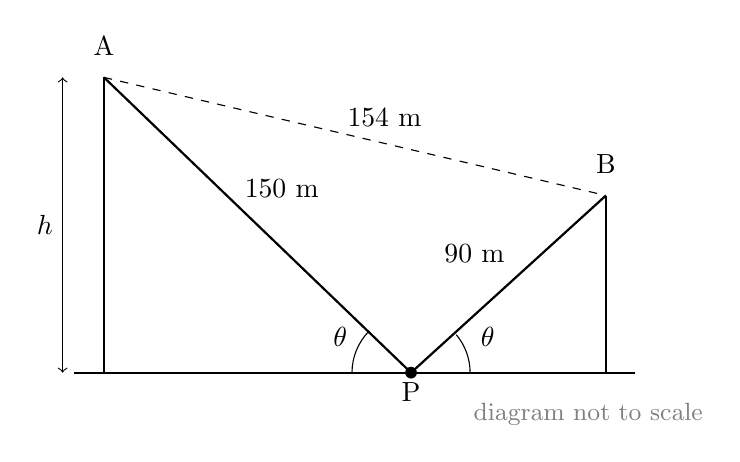
\begin{tikzpicture}[scale=0.75]
% Ground line
\draw[thick] (-0.5,0) -- (9,0);
% Taller building (left)
\draw[thick] (0,0) -- (0,5);
\node[above] at (0,5.2) {A};
% Shorter building (right)
\draw[thick] (8.5,0) -- (8.5,3);
\node[above] at (8.5,3.2) {B};
% Point P
\node[below] at (5.2,0) {P};
\node[fill=black, circle, inner sep=1.5pt] at (5.2,0) {};
% Lines from P to tops
\draw[thick] (5.2,0) -- (0,5);
\draw[thick] (5.2,0) -- (8.5,3);
% Labels
\node[above left] at (3.8,2.8) {150 m};
\node[above right] at (5.6,1.7) {90 m};
\draw[dashed] (0,5) -- (8.5,3);
\node[above] at (4.75,4.) {154 m};
% Height h
\draw[<->] (-0.7,0) -- (-0.7,5);
\node[left] at (-0.7,2.5) {$h$};
% Angle theta at P (left)
\draw (5.2,0) ++(180:1) arc (180:135:1);
\node at (4.,0.6) {$\theta$};
% Angle theta at P (right)
\draw (5.2,0) ++(40:1) arc (40:0:1);
\node at (6.5,0.6) {$\theta$};
% Not to scale
\node[gray] at (8.2,-0.7) {\small diagram not to scale};
\end{tikzpicture}
\end{center}
\vspace{-0.3cm}

The distance from point P to point A is 150\,m. \\
The distance from point P to point B is 90\,m. \\
The distance between A and B is 154\,m.

\begin{enumerate}[itemsep=0.1cm]
  \item[(a)] Find the measure of $A\hat{P}B$. \hfill [3]
  \item[(b)] Find the height, $h$, of the taller building. \hfill [3]
\end{enumerate}

\begin{tikzpicture}
  \draw (-0.6,0) rectangle (11,7);
  \foreach \y in {1,2,...,6} \draw[dotted] (0,\y)--(10.5,\y);
\end{tikzpicture}

\newpage

%--- Problem 5: Ferris wheel [5 marks] ---
\item[5.] [Maximum mark: 5]

A Ferris wheel with diameter 110 metres rotates at a constant speed. The lowest
point on the wheel is 10 metres above the ground. P is a point on the wheel. The wheel
starts moving with P at the lowest point and completes one revolution in 20 minutes.

\begin{center}
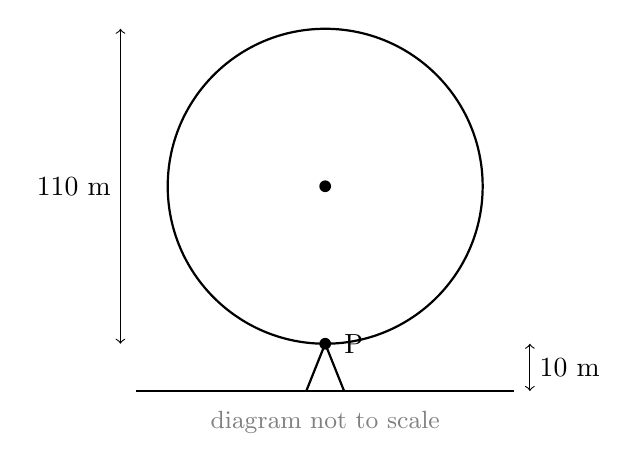
\begin{tikzpicture}[scale=0.4]
% Ground
\draw[thick] (-6,0) -- (6,0);
% Wheel
\draw[thick] (0,6.5) circle (5);
\node[fill=black, circle, inner sep=1.5pt] at (0,6.5) {};
% Point P
\node[fill=black, circle, inner sep=1.5pt] at (0,1.5) {};
\node[right] at (0.3,1.5) {P};
% Support
\draw[thick] (-0.6,0) -- (0,1.5) -- (0.6,0);
% Diameter label
\draw[<->] (-6.5,1.5) -- (-6.5,11.5);
\node[left] at (-6.5,6.5) {110 m};
% 10m label
\draw[<->] (6.5,0) -- (6.5,1.5);
\node[right] at (6.5,0.75) {10 m};
\node[gray] at (0,-1) {\small diagram not to scale};
\end{tikzpicture}
\end{center}
\vspace{-0.3cm}

The height, $h$ metres, of P above the ground after $t$ minutes is given by
$h(t) = a\cos(bt) + c$, where $a, b, c \in \mathbb{R}$.

Find the values of $a$, $b$ and $c$.

\begin{tikzpicture}
  \draw (-0.6,0) rectangle (11,9);
  \foreach \y in {1,2,...,8} \draw[dotted] (0,\y)--(10.5,\y);
\end{tikzpicture}

\newpage

%--- Problem 6: Drug decay [5 marks] ---
\item[6.] [Maximum mark: 5]

The amount of a drug, in milligrams (mg), in a patient's body can be modelled by
the function $A(t) = 500e^{-kt}$, where $k$ is a positive constant and $t$ is the
time in hours after the initial dose is given.

\begin{enumerate}[itemsep=0.1cm]
  \item[(a)] Write down the amount of the drug in the patient's body when $t = 0$. \hfill [1]
\end{enumerate}

After three hours, the amount of the drug in the patient's body has decreased to 280\,mg.

\begin{enumerate}[itemsep=0.1cm]
  \item[(b)] Find the value of $k$. \hfill [2]
\end{enumerate}

The second dose is given $T$ hours after the initial dose, when the amount of the drug
in the patient's body is 140\,mg.

\begin{enumerate}[itemsep=0.1cm]
  \item[(c)] Find the value of $T$. \hfill [2]
\end{enumerate}

\begin{tikzpicture}
  \draw (-0.6,0) rectangle (11,10);
  \foreach \y in {1,2,...,9} \draw[dotted] (0,\y)--(10.5,\y);
\end{tikzpicture}

\newpage

%--- Problem 7: Carbon-14 [7 marks] ---
\item[7.] [Maximum mark: 7]

All living plants contain an isotope of carbon called carbon-14. When a plant dies,
the isotope decays so that the amount of carbon-14 present decreases. The amount, $A$,
of carbon-14 present $t$ years after death can be modelled by $A = A_0 e^{-kt}$
where $t \geq 0$ and $A_0$, $k$ are positive constants.

At the time of death, a plant is defined to have 100 units of carbon-14.

\begin{enumerate}[itemsep=0.1cm]
  \item[(a)] Show that $A_0 = 100$. \hfill [1]
\end{enumerate}

The time taken for half the original amount of carbon-14 to decay is known to be 5730 years.

\begin{enumerate}[itemsep=0.1cm]
  \item[(b)] Show that $k = \dfrac{\ln 2}{5730}$. \hfill [3]
  \item[(c)] Find, correct to the nearest 10 years, the time taken after the plant's death
  for 25\% of the carbon-14 to decay. \hfill [3]
\end{enumerate}

\begin{tikzpicture}
  \draw (-0.6,0) rectangle (11,9);
  \foreach \y in {1,2,...,8} \draw[dotted] (0,\y)--(10.5,\y);
\end{tikzpicture}

\newpage

%--- Problem 8: Kinematics [7 marks] ---
\item[8.] [Maximum mark: 7]

A particle moves in a straight line such that its velocity, $v$ m\,s$^{-1}$, at
time $t$ seconds is given by
\[v = \frac{(t^2 + 1)\cos t}{4}, \quad 0 \leq t \leq 3.\]

\begin{enumerate}[itemsep=0.1cm]
  \item[(a)] Determine when the particle changes its direction of motion. \hfill [2]
  \item[(b)] Find the times when the particle's acceleration is $-1.9$ m\,s$^{-2}$. \hfill [3]
  \item[(c)] Find the particle's acceleration when its speed is at its greatest. \hfill [2]
\end{enumerate}

\begin{tikzpicture}
  \draw (-0.6,0) rectangle (11,13);
  \foreach \y in {1,2,...,12} \draw[dotted] (0,\y)--(10.5,\y);
\end{tikzpicture}

\newpage

%--- Problem 9: Kinematics with graph [6 marks] ---
\item[9.] A particle moves in a straight line such that its velocity, $v$ m\,s$^{-1}$, at
time $t$ seconds is given by
\[v(t) = 4e^{-t/3}\cos\!\left(\frac{t}{2} - \frac{\pi}{4}\right),
\quad \text{for } 0 \leq t \leq 4\pi.\]
The graph of $v$ is shown in the following diagram.

\begin{center}
\begin{tikzpicture}
\begin{axis}[
    width=9cm, height=5.5cm,
    axis lines=middle,
    xlabel={$t$}, ylabel={$v(t)$},
    xmin=-0.5, xmax=13.5,
    ymin=-0.5, ymax=3.5,
    xtick={12.56637},
    xticklabels={$4\pi$},
    ytick=\empty,
    tick label style={font=\small},
    every axis x label/.style={at={(ticklabel* cs:1)}, anchor=west},
    every axis y label/.style={at={(ticklabel* cs:1)}, anchor=south},
]
\addplot[thick, domain=0:12.57, samples=300]
    {4*exp(-x/3)*cos(deg(x/2 - pi/4))};
\end{axis}
\end{tikzpicture}
\end{center}
\vspace{-0.3cm}

Let $t_1$ be the first time when the particle's \emph{acceleration} is zero.

\begin{enumerate}[itemsep=0.1cm]
  \item[(a)] Find the value of $t_1$. \hfill [2]
\end{enumerate}

Let $t_2$ be the \emph{second} time when the particle is instantaneously at rest.

\begin{enumerate}[itemsep=0.1cm]
  \item[(b)] Find the value of $t_2$. \hfill [2]
  \item[(c)] Find the distance travelled by the particle between $t = t_1$ and
  $t = t_2$. \hfill [2]
\end{enumerate}

\begin{tikzpicture}
  \draw (-0.6,0) rectangle (11,11);
  \foreach \y in {1,2,...,10} \draw[dotted] (0,\y)--(10.5,\y);
\end{tikzpicture}

\end{enumerate}
\end{document}

Solutions
  Problem 1 — Regression (GDC):
  (a) a = 1.93, b = 7.22
  (b) r = 0.991
  (c) h = 1.93(20) + 7.22 = 45.9 cm

  Problem 2 — Compound interest:
  (a) 1700(1 + 0.0274/2)^20 = $2231.71
  (b) 1700(1 + r/100)^10 = 2231.71 → r = 2.76
  (c) Interest = 2231.71 - 1700 = $531.71

  Problem 3 — Geometric sequence:
  50r³ = 86.4, r = 1.2
  S_n = 250(1.2^n - 1) > 33500
  S_26 = 28368.8, S_27 = 34092.6 → n = 27

  Problem 4 — Buildings:
  (a) Cosine rule: 154² = 150² + 90² - 2(150)(90)cos(∠APB) → ∠APB = 75.2°
  (b) θ = (180 - 75.2)/2 = 52.4°, h = 150 sin(52.4°) = 119 m

  Problem 5 — Ferris wheel:
  a = -55 (starts at bottom), c = 10 + 55 = 65 (centre height)
  2π/b = 20 → b = π/10

  Problem 6 — Drug decay:
  (a) A(0) = 500 mg
  (b) 280 = 500e^(-3k) → k = -(1/3)ln(280/500) = 0.193
  (c) 500e^(-0.193T) = 140 → T = 6.59 hours

  Problem 7 — Carbon-14:
  (a) At t = 0: A = A₀e⁰ = A₀ = 100
  (b) 50 = 100e^(-5730k) → e^(-5730k) = 1/2 → k = ln2/5730
  (c) 25% decayed → 75 remains: 75 = 100e^(-(ln2/5730)t) → t = 2380 years

  Problem 8 — Kinematics:
  (a) v = 0 when cos t = 0 → t = π/2 = 1.57 s
  (b) GDC: v'(t) = -1.9 → t = 2.26 s and t = 2.96 s
  (c) GDC: max |v| at t = 3, a(3) = v'(3) = -1.84 m/s²

  Problem 9 — Kinematics:
  (a) GDC: v'(t) = 0 → t₁ = 0.395 s
  (b) v(t) = 0: first zero t = 3π/2, second zero t₂ = 7π/2 = 11.0 s
  (c) ∫|v|dt from t₁ to t₂ = 6.54 + 1.29 = 7.83 m
